%%%%%%%%%%%%%%%%%%%%%%%%%%%%%%%%%%%%%%%%%
% University Assignment Title Page 
% LaTeX Template
% Version 2.1 (18/10/18)
% Modified by
% Erdem TUNA &
% Halil TEMURTAŞ &
% Enes TAŞTAN
%%%%%%%%%%%%%%%%%%%%%%%%%%%%%%%%%%%%%%%%%
%
%----------------------------------------------------------------------------------------
%	PACKAGES AND OTHER DOCUMENT CONFIGURATIONS
%----------------------------------------------------------------------------------------
\documentclass[a4paper,12pt]{article}
%-----packages------
\usepackage[a4paper, total={6.2in, 9in}]{geometry}
\usepackage[english]{babel}
\usepackage[utf8x]{inputenc}
\usepackage{amsmath}
\usepackage{graphicx}
\usepackage[colorinlistoftodos]{todonotes}
\usepackage{gensymb} % this could be problem
\usepackage{float}
\usepackage{fancyref}
\usepackage{subcaption}
\usepackage[titletoc]{appendix} %appendix package
\usepackage{xcolor}
\usepackage{listings}
\usepackage{xspace}
\usepackage{amssymb}
\usepackage{nicefrac}
\usepackage{gensymb}
\usepackage{fancyhdr}
\usepackage{lipsum}  % for dummy text \lipsum[1-4]
\usepackage[final]{pdfpages}  % pdf include
%\usepackage{array} %allows more options in tables
\usepackage{pgfplots,pgf,tikz} %coding plots in latex
%\usepackage{capt-of} % allows caption outside the figure environment
\usepackage[export]{adjustbox} %more options for adjusting the images
%\usepackage{multicol,multirow,slashbox} % allows tables like table1
%\usepackage[hyperfootnotes=false]{hyperref} % clickable references
%\usepackage{epstopdf} % useful when matlab is involved
%\usepackage{placeins} % prevents the text after figure to go above figure with \FloatBarrier 
%\usepackage{listingsutf8,mcode} %import .m or any other code file mcode is for matlab highlighting
\usepackage{setspace}
%-----end of packages




%-----specifications-----
\definecolor{mGreen}{rgb}{0,0.6,0} % for python
\definecolor{mGray}{rgb}{0.5,0.5,0.5}
\definecolor{mPurple}{rgb}{0.58,0,0.82}
\definecolor{mygreen}{RGB}{28,172,0} % color values Red, Green, Blue for matlab
\definecolor{mylilas}{RGB}{170,55,241}

\setcounter{secnumdepth}{5} % how many sectioning levels to assign numbers to
\setcounter{tocdepth}{5}    % how many sectioning levels to show in ToC

\lstdefinestyle{CStyle}{
	commentstyle=\color{mGreen},
	keywordstyle=\color{magenta},
	numberstyle=\tiny\color{mGray},
	stringstyle=\color{mPurple},
	basicstyle=\footnotesize,
	breakatwhitespace=false,         
	breaklines=true,
	frame=single,
	rulecolor=\color{black!40},                 
	captionpos=b,                    
	keepspaces=true,                 
	numbers=left,                    
	numbersep=5pt,                  
	showspaces=false,                
	showstringspaces=false,
	showtabs=false,                  
	tabsize=2,
	language=C
}

\lstset{language=Matlab,%
	%basicstyle=\color{red},
	breaklines=true,%
	frame=single,
	rulecolor=\color{black!40},
	morekeywords={matlab2tikz},
	keywordstyle=\color{blue},%
	morekeywords=[2]{1}, keywordstyle=[2]{\color{black}},
	identifierstyle=\color{black},%
	stringstyle=\color{mylilas},
	commentstyle=\color{mygreen},%
	showstringspaces=false,%without this there will be a symbol in the places where there is a space
	numbers=left,%
	numberstyle={\tiny \color{black}},% size of the numbers
	numbersep=9pt, % this defines how far the numbers are from the text
	emph=[1]{for,end,break},emphstyle=[1]\color{red}, %some words to emphasise
	%emph=[2]{word1,word2}, emphstyle=[2]{style},    
}


\tikzset{
	desicion/.style={
		diamond,
		draw,
		text width=4em,
		text badly centered,
		inner sep=0pt
	},
	block/.style={
		rectangle,
		draw,
		text width=10em,
		text centered,
		rounded corners
	},
	cloud/.style={
		draw,
		ellipse,
		minimum height=2em
	},
	descr/.style={
		fill=white,
		inner sep=2.5pt
	},
	connector/.style={
		-latex,
		font=\scriptsize
	},
	rectangle connector/.style={
		connector,
		to path={(\tikztostart) -- ++(#1,0pt) \tikztonodes |- (\tikztotarget) },
		pos=0.5
	},
	rectangle connector/.default=-2cm,
	straight connector/.style={
		connector,
		to path=--(\tikztotarget) \tikztonodes
	}
}

\tikzset{
	desicion/.style={
		diamond,
		draw,
		text width=4em,
		text badly centered,
		inner sep=0pt
	},
	block/.style={
		rectangle,
		draw,
		text width=10em,
		text centered,
		rounded corners
	},
	cloud/.style={
		draw,
		ellipse,
		minimum height=2em
	},
	descr/.style={
		fill=white,
		inner sep=2.5pt
	},
	connector/.style={
		-latex,
		font=\scriptsize
	},
	rectangle connector/.style={
		connector,
		to path={(\tikztostart) -- ++(#1,0pt) \tikztonodes |- (\tikztotarget) },
		pos=0.5
	},
	rectangle connector/.default=-2cm,
	straight connector/.style={
		connector,
		to path=--(\tikztotarget) \tikztonodes
	}
}
%-----end of specifications-----


%----commands----
\newcommand\nd{\textsuperscript{nd}\xspace}
\newcommand\rd{\textsuperscript{rd}\xspace}
\newcommand\nth{\textsuperscript{th}\xspace} %\th is taken already
\newcommand{\specialcell}[2][c]{ \begin{tabular}[#1]{@{}c@{}}#2\end{tabular}} % for too long table lines

\newcommand{\blankpage}{
	\- \\[9.5cm]	
	{ \centering \textit{This page intentionally left blank.} \par }
	\- \\[9.5cm]
}% For Blank Page

\makeatletter
\renewcommand\paragraph{\@startsection{paragraph}{4}{\z@}%
	{-2.5ex\@plus -1ex \@minus -.25ex}%
	{1.25ex \@plus .25ex}%
	{\normalfont\normalsize\bfseries}}
\makeatother
%-----end of commands-----
%\onehalfspacing
\begin{document}

\begin{titlepage}

\newcommand{\HRule}{\rule{\linewidth}{0.5mm}} % Defines a new command for the horizontal lines, change thickness here
\centering 


\includegraphics[width=\textwidth,height=\textheight,keepaspectratio]{../../documents/logos/logo3-with-stroke}\\[0.5cm]

\textsc{\LARGE Middle East Technical University}\\[0.5cm] % Name of your university/college
\textsc{\Large Department of \\Electrical and Electronics Engineering }\\[0.5cm] % Major heading such as course name
\textsc{\large EE493 ENGINEERING DESIGN I}\\[0.5cm] % Minor heading such as course title


\HRule \\[0cm]
{ \huge \bfseries  Car Chasing Robot\\[0.1cm] \LARGE \bfseries Conceptual Design Report}\\[0cm] % Title of your document
\HRule \\[1cm]

\begin{minipage}[l]{0.6\textwidth}
\raggedright
		\large{\textbf{Supervisor:}}	Assoc. Prof. Emre Özkan \\
		\hspace{3.05cm}  METU EE / C-112

\end{minipage}
\begin{minipage}[r]{0.35\textwidth}
\raggedright
		\textbf{Project Start:} 4/10/2018\\
		\textbf{Project End:} \ \  26/5/2019\\
		\textbf{Project Budget:} \$450

\end{minipage}\\[1cm]
\begin{minipage}{\textwidth}
	\begin{flushleft}
		\large{\textbf{Company Name :}}	Duayenler Ltd. Şti.\\
		\begin{table}[H]
			\begin{tabular}{l l l l}
				\hline
				\textbf{Members}&\textbf{Title}& \textbf{ID}&\textbf{Phone} \\ \hline
				Sarper Sertel & Electronics Engineer& 2094449 & 0542 515 6039  \\ 
				Enes Taştan & Hardware Design Engineer & 2068989 & 0543 683 4336  \\ 
				Erdem Tuna & Embedded Systems Engineer& 2617419 & 0535 256 3320  \\ 
				Halil Temurtaş & Control Engineer& 2094522 & 0531 632 2194  \\
				İlker Sağlık & Software Engineer& 2094423 & 0541 722 9573  \\ \hline
				
				
			\end{tabular}
		\end{table}
	\end{flushleft}
\end{minipage}\\[1cm]

\begin{flushbottom}
{\large December 26, 2018} % Date, change the \today to a set date if you want to be precise
\end{flushbottom}

\end{titlepage}

\blankpage
\tableofcontents
\newpage

\section{Executive Summary}

	

\section{Introduction}
	DUAYENLER is established with the aim of developing autonomous car technologies for near future. To serve that purpose,  Car Chasing Project is initiated by the company. The project can be summarized as a vehicle that can autonomously follow a path and detect the other surrounding vehicle as well as communicating them to have a reliable driving environment.  With this project, the company aims to accomplish the following objectives:
	\begin{enumerate}
		\item Sensing the environment and other vehicles on the roads
		\item Automatic adaptive lane detection
		\item Self driving
		\item Autonomous wireless communication with surrounding counterparts		
	\end{enumerate}
	
	A considerable amount of effort and work force has been put on the project to fulfill the required objectives. So far, the team has figured out several important steps towards the realization of the project.To start with, the wireless communication between the vehicles is modeled and implemented. A reliable communication environment is established using Wi-Fi protocol. Currently, the vehicles can communicate with each others by means of associated handshake protocol messages in a race scenario. Secondly, computer vision algorithms are developed and implemented as a solution to lane detection problem. The algorithms are developed based on open source computer vision library OpenCV. To obtain a direction predicting results, color thresholding, edge detection, hough transform algorithms are used respectively. Furthermore, the communication between image processing platform and microcontrollers for motor driving is constructed. It is the essential part of solving the self driving problem. On the mechanical part, different motor\&wheel combinations are tested to obtain the best performance. To test the computer vision on board, a prototype vehicle is assembled and necessary equipment is mounted on it. Currently, the team is working on the improvement of computer vision algorithms.\\
	
	In this report, the company provides technical details about the implemented solutions, other possible solution alternatives with objective comparisons as well as a clear action plan showing the necessary further steps for realization of the project. The emphasis on this report is primarily put on the detailed analysis of proposed solutions, supported with relevant test results in both system and subsystem level. In addition, future plans including new test designs for current solutions as well as for other alternatives, the action plan in case of unexpected outcomes by clearly specifying the responsibilities of each member in the team. \\
	


\begin{figure}[H]
\center
\setlength{\unitlength}{\textwidth} 
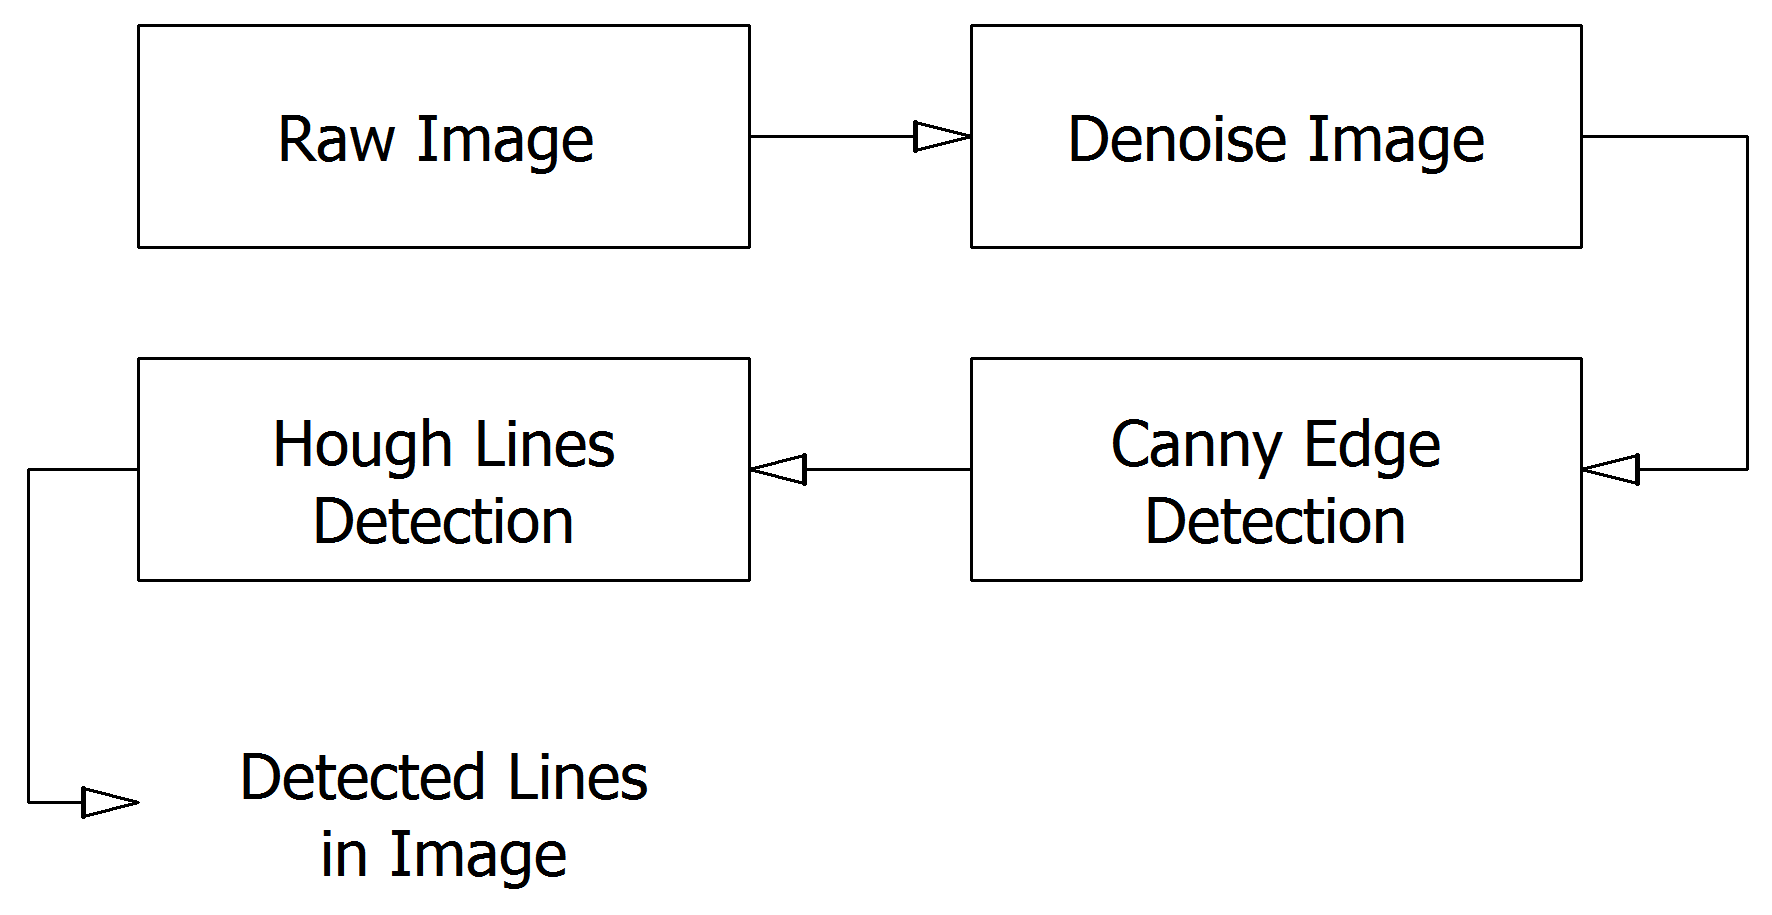
\includegraphics[width=\textwidth]{v-models/lane_detection_subsystem}
\caption{\label{fig:lane_detection_subsystem}The Proposed Algorithm for the Lane Detection.}
\end{figure}
\section{Solutions}

	\subsection{Description of individual sub-systems}

	\subsubsection{Sensing System}
<<<<<<< HEAD
		Sensing system has two main subsystems which are "Lane Detection Subsystem" and "Vehicle Detection Subsystem".
=======
		This unit has two main subsystems which are observing lane and another vehicle on the path. 
>>>>>>> 2ca5b1cc4ec65f41c061efad317265ce5c62fce8
		
		\paragraph{Lane Detection Subsystem}
			The subsystem basically detects the lane. This subsystem uses OpenCV libraries for processing camera frames. The input is captured from a Raspberry Pi camera that is mounted to the vehicle. The captured frame is firstly, preprocessed by a denoising filter. Then, the edges in the frame is detected by Canny Edge Detector algorithm. The output of Canny is a binary image filled with ones and zeros. The Hough Lines technique probabilistically extracts possible lines in a given binary image. Thus, possible line constituting points are obtained from Hough Lines function. Next, points of the lines are classified as left or right borders of the lane. The elimination of the wrong points are done concurrently with the classification. Then, filtered points are fitted in two separate lines to create left and right borders of the lane. As the lane borders are found, the next and the last step is to determine the direction of the vehicle. The output of this subsystem is a turning angle and a direction.

		\paragraph{Vehicle Detection Subsystem}
			The detection of the opponent can be implemented using distance sensors. In order to stop the robot when it catches the opponent, or it is caught, a sensor must be placed at the front and the back. The most common distance sensors are ultrasonic, infrared and laser sensors. 

Ultrasonic sensors have acceptable range. They send a sound wave and take back the echo, then give a PWM voltage related to the distance. However, using ultrasonic sensors can cause problems if the opponent also uses ultrasonic sensors; because of the interference. Besides, when measurement is angled, measuring is failing. 

Infrared sensors can be another approach to this problem, they may provide better accuracy. Moreover, Laser distance measurement can be applied to solve this problem. They have the best accuracy, but their price is the highest among the rest.

	\subsubsection{Computation System}
		Functionality of computation subsystem will be presented in this section.
	
		\paragraph{Data Processing Subsystem}
		This unit is the main algorithm application level. Data from sensor will be aggregated in this unit and will be pre-processed. Then, processed data will be output to the controller unit. Processing will mainly be done using Arduino and Raspberry Pi (if used). Suitable algorithms will be developed to realize desired operations with the controller unit

		\paragraph{Controller Subsystem}
			Mathematical models will be implemented in this unit to realize controllers such as P, PI, PID. The output of the controller unit will be sent to driving subsystem. This output will be the ultimate decision to realize a desired operation according to the data sent from sensor.


	\subsubsection{Communication System}
	
		\paragraph{Internal Communication Subsystem}
		
		\paragraph{External Communication Subsystem}
		
		
	\subsubsection{Driving System}
		This unit takes an input from the controller unit. That input involves information about what the new orientation should be. Driving subsystem, then, takes action to move vehicle according to the required direction with maximum possible speed. This subsystem consists of two units: Direction and Speed.

		\paragraph{Direction Subsystem}
			Direction unit is responsible for the orientation of the vehicle. It stores the last required orientation and the new one coming from the controller. After that, it tries to make the orientation as close as new one. Both data can be represented as vectors.The angle between those two vector is tried to be minimized by the controller. Before moving on to the operation, note that the angle can be used as a measure of the error that the direction unit have. The less the angle the more correctly operates the direction unit.\\

			Depending on the configuration of the wheels, exact control of the vehicle might vary. However, there are certain methods to accomplish orientation. The vehicle will definitely have two wheels or palettes that will be driven by two separate DC motors. That configuration allows differential drive method to orient the vehicle. PWM values of the motors can be adjusted such that the speed difference between them results in a turn as much as desired angle. The exact difference values on the PWM values depends on the specs of the used motors and voltage sources. \\

			Two different H-bridge motor drivers are proposed to be used to drive DC motors: L298N and L293D. Both can drive two motors separately with one IC. However, maximum current rating of the former one is larger being 2A while L293D can supply 0.6A per channel. \\

			As in the case of another configuration that involves one or two servo motors to control the directions of the front wheels. This configuration is more robust compared to ball caster utilization. However, there are more motors to control and it requires more complicated differential drive algorithms involving both DC motor differential and servo PWM to orient the front wheels.
		\paragraph{Speed Unit}

		This unit acts as a complementary module for direction unit. It will act as a state machine. In one state, the unit will try to increase the speed of the vehicle by making overall increase in both PWM values of DC motors. The feedback of this  system will be the cost function mentioned in driving unit. If that cost exceeds a specified level, unit goes to another state in which the unit will decrease the overall speed to allow direction unit to operate more correctly. In short, this unit tries to compensate the error of the direction unit by changing the overall speed of the vehicle.
 

	\subsubsection{Structure Subsystem}
		This part contains chassis and PCB sections of the robot. 
		
		\paragraph{Chassis Subsystem}
			Main purposes of this section are protection of the critical elements of the robot and holding components together. The most important part of this section is weight distribution. The chassis is supposed to be light and strong because of the competition purposes. However, it should balance the robot to be able to handle with turns. 
		\paragraph{Printed Circuit Board Subsystem}
			The main role of this part is decreasing connection mass and increase vibration strength of the robot against disturbances. Also, this section increases rigidity of the whole system. 
	
	
	\subsubsection{Motion System}
		Motion of the system is detailed in this section.
		\paragraph{Wheels Subsystem}
			There are possible solution for wheel placement on the chassis, and several wheel types. Some wheels are designed for better gripping on different surfaces. To avoids obstacles on the path, gripping of the wheel is an important concept. Some wheel types are ball caster, toy car wheel and palette. Besides, wheel placement and the wheel number should be combined with the wheel type choice. \\
	
			One of the possible wheel placement is 2+1 combination. This combination can be assembled by placing 2 car wheels (with motors) to the back and the one boll caster to the front or vice versa. These configurations provide easy implementation and fairly reliable handling on the path. However, for certain obstacles may significantly disturb vehicles balance in this configuration.\\

			Another combination is palette system. This system is used in real world where robust vehicles are needed. Similarly, this configuration can help handling obstacle in the path, but it costs for harder implementation and driving.\\

Last implementation is 2+2 configuration. In this configuration 2 wheels can be placed at the back and the rest at the front by placing motors to back wheels. To ease turning of the vehicle, front wheels can be controlled with a servo motor as back wheels operate in the differential drive mode. This combination may provide both enhanced grip and reliable	 operation. \\
		\paragraph{Motors Subsystem}
			Motors are one of the most important physical components of the project. There are possible motor types in the market.\\

			One of the widely used motor type is brushed DC motors. Such motors might be implemented with gears. Gears are utilized to adjust torque and RPM of the motor, which is very suitable for a racing vehicle's needs. \\

			Another option is brushless DC motors. Brushless DC motors do not use brushes. This results in high torque. Brushless motors are more suitable for high RPM required areas such as CD drivers and drones.\\

			Last option is servo motors. Servo motors are high-torque motors that can turn in an desired angle. Servos can be utilized in the direction of the vehicle on the front wheels. By using this solution, turning radius can be decrease significantly.\\

\subsection{System \& Subsystem Level Requirements}
		
	
	\subsubsection{Sensing System Requirements}
	
		\begin{itemize}
			\item The system should detect the sides of the road.
			\item The system should not be effected from external disturbances.
			\item The system should detect the opponent vehicle.
		\end{itemize}

	\paragraph{Lane Detection Subsystem Requirements}	
		
		\begin{itemize}
			\item The subsystem should be able to detect only the shades of green color
			\item The subsystem should be able to detect edges in the camera frame in any light condition
			\item The subsystem should be able to tell differences between disturbances and lane
			\item The subsystem should be able to interpret the middle of the lane if both sides are present at the frame
		\end{itemize}
	 
	 
	\paragraph{Vehicle Detection Subsystem Requirements}
	
		\begin{itemize}
			\item The subsystem should detect the opponent to be caught with in a 5 cm 
			\item The subsystem should detect the chasing opponent if it reaches from back with in a 5 cm  
		\end{itemize}
		
		
	\subsubsection{Computation System Requirements}
		
		\begin{itemize}
			\item The system should	be able to produce middle line to follow
			\item The system should be able to control the robot
		\end{itemize}			
	
	
	\paragraph{Data Processing Subsystem Requirements}	
	
		\begin{itemize}
			\item The subsystem should be able to analyse data produced by sensing system
			\item The subsystem should be able to produce the angle information required by the controller subsystem
			\item The subsystem should be able to work on Raspberry Pi
			\item The subsystem should be able to process one frame at most in 100 milliseconds
		\end{itemize}
		
	\paragraph{PID Controller Subsystem Requirements}
	
		\begin{itemize}
			\item The subsystem should be able to control the motors
			\item The subsystem should be able to react the external disturbances
		\end{itemize}
	
	\subsubsection{Communication System Requirements}
		
		\begin{itemize}
			\item The subsystem should ensure safe internal communication
			\item The subsystem should ensure safe external communication
		\end{itemize}
	
	\paragraph{Internal Communication Subsystem Requirements}

		\begin{itemize}
			\item The microcontrollers should be able to communicate with each other via serial communication
			\item The internal communication speed should be compatible with the processing speed of the lane detection subsystem  
		\end{itemize}
	
	\paragraph{External Communication Subsystem Requirements}	
	
		\begin{itemize}
			\item The subsystem should be able to communicate with the opponent via Wi-fi protocol
			\item The subsystem should be able to execute handshake protocol
		\end{itemize}
	
	
	\subsubsection{Driving System Requirements}
	
		\begin{itemize}
			\item The subsystem should control motion subsystem according to output of the computation system
		\end{itemize}
	
	\paragraph{Speed Subsystem Requirements}	
		
		\begin{itemize}
			\item The subsystem should decrease the vehicle speed at the narrow lane 
			\item The subsystem should increase the vehicle speed at the wide lane 
			\item The subsystem should decrease the vehicle speed at the extreme disturbance  
		\end{itemize}
		
	\paragraph{Direction Subsystem Requirements}
	
		\begin{itemize}
			\item The subsystem should drive the motors according to computation system outputs
			\item The system should ensure that the vehicle follows the lane 
		\end{itemize}


	\subsubsection{Motion System Requirements}
	
		\begin{itemize}
			\item The system should	ensure that the vehicle can drive itself with enough power
		\end{itemize}
	
	\paragraph{Wheels Subsystem Requirements}	
		
		\begin{itemize}
			\item The subsystem should ensure that the wheels can grip lane without slipping in all conditions 	
		\end{itemize}
		
	\paragraph{Motors Subsystem Requirements}
	
		\begin{itemize}
			\item The subsystem should ensure that the motors can supply enough torque to accelerate the vehicle		
			\item  The subsystem should ensure that the motors can execute driving system outputs without deviation 
		\end{itemize}
	
	
	\subsubsection{Structure System Requirements}
	
		\begin{itemize}
			\item The system should	ensure that structure is robust for external effects 
			\item The system should	ensure that structure is balanced to increase handling
	
		\end{itemize}
	
	\paragraph{Chasis Subsystem Requirements}	
		
			\begin{itemize}
			\item The subsystem should ensure that the chassis is rigid 
			\item The subsystem should ensure that the chassis have enough space for components
			\item The subsystem should ensure that the chassis can provide low center of mass 

		\end{itemize}
		
	\paragraph{PCB Subsystem Requirements}
	
		\begin{itemize}
			\item The subsystem should ensure that all the electronic devices are placed on PCB
			\item The subsystem should ensure that the components are not connected via loose cable 	
		\end{itemize}	



	



	\subsection{Solution for each subsystem and relevant algorithms}
	
	
	\subsection{Subsystem level risk assessment, and alternative solutions (Plan-B)}
	
	
	\subsection{ Error sources, their impact and ways to mitigate}
	
	
	\subsection{System \& Subsystem Tests }
	

	\subsubsection{Sensing System Tests}
	
		

	\paragraph{Lane Detection Subsystem Tests}	
	
		\paragraph{Light Condition Test}
		
		\paragraph{Visual Disturbance Test}
		
		\paragraph{}
	 
	 
	\paragraph{Vehicle Detection Subsystem Tests}
	
		\paragraph{•}
	\subsubsection{Computation System Tests}
	
	\paragraph{Data Processing Subsystem Tests}	
		
	\paragraph{PID Controller Subsystem Tests}
	
	
	\subsubsection{Driving System Tests}
	
	\paragraph{Speed Subsystem Tests}	
		
	\paragraph{Direction Subsystem Tests}


	\subsubsection{Motion System Tests}
	
	\paragraph{Wheels Subsystem Tests}	
		
	\paragraph{Motors Subsystem Tests}
	
	
	\subsubsection{Structure System Tests}
	
	\paragraph{Chasis Subsystem Tests}	
		
	\paragraph{PCB Subsystem Tests}
	
	
	\subsection{Technical drawing of the expected design}
	

\section{Plans}


\section{Conclusion}



\section{Disclaimer}


\end{document}

%----samples------
%\begin{itemize}
%\item Item
%\item Item
%\end{itemize}

%\begin{figure}[H]
%\center
%\setlength{\unitlength}{\textwidth} 
%
\includegraphics[width=0.7\unitlength]{images/logo1}
%\caption{\label{fig:logo}Logo }
%\end{figure}

%\begin{figure}[H]
%	\setlength{\unitlength}{\textwidth} 
%	\centering
%	\begin{subfigure}{.5\textwidth}
%  		\centering
%  		
\includegraphics[width=0.48\unitlength]{images/logo1}
%  		\caption{\label{fig:logo1}Logo1 }
%	\end{subfigure}%
%	\begin{subfigure}{.5\textwidth}
%  		\centering
%		
\includegraphics[width=0.48\unitlength]{images/logo2}
%  		\caption{\label{fig:logo2}Logo2}
%	\end{subfigure}
%\caption{\label{fig:calisandegree} Small Logos   }
%\end{figure}
	
%\begin{table}[H]
%  \centering
% 
%    \begin{tabular}{c|c|c}
%       $$A$$ & $$B$$ & $$C$$ \\ \hline
%       1 & 2 & 3  \\ \hline
%       2 & 3 & 4  \\ \hline
%       3 & 4 & 5  \\ \hline
%       4 & 5 & 6  
%      
%  \end{tabular}
%  \caption{table}
%  \label{tab:table}
%\end{table}
	
%\begin{table}[H]
%  \centering
% 
%    \begin{tabular}{c|c|c}
%       \backslashbox{$A$}{$a$} & $$\specialcell{ Average deviation \\ after subtracting out the  \\ frequency error }$$ & $$C$$ \\ \hline
%       \multirow{2}{*}{1} & 2 & 3  \\ \cline{2-3}
%        & 3 & 4  \\ \hline
%       3 & \multicolumn{2}{c}{4}  \\ \hline
%       4 & 5 & 6  
%      
%  \end{tabular}
%  \caption{table}
%  \label{tab:table}
%\end{table}
%-----end of samples-----